\chapter{Implementierung}
%
Ursprünglich war der Ansatz, ein eigenständiges Programm zu entwickeln, welches selbstständig Wasserzeichen auf Bildern platziert. Dabei sollten die Gesichter ausgespart werden, um die Ästhetik des Bildes nicht zu stören. Aufgrund der limitierten Zeit wird dieser Ansatz auf das Markieren von Gesichtsbereichen reduziert. Diese Reduktion erlaubt eine flexiblere Implementierung, indem statt eines eigenständigen Programms ein Modul erstellt wird. Damit ergeben sich mehr Anwendungsmöglichkeiten, die über das einfache Platzieren von Wasserzeichen hinaus gehen.

Bisher wurde für das Laden der Bilder in dieser Arbeit \texttt{cv2} genutzt, genauer die Funktion \texttt{cv2.imread()}, welche Bilder im BGR-Format lädt. Bei der Implementierung ist allerdings aufgefallen, dass diese Funktion Probleme mit Umlauten hat. Aus diesem Grund wurde auf die Funktion \texttt{Image.open().convert("RGB")} von PIL gewechselt. Bemerkenswert ist, dass RetinaFace mit RGB-Input weniger False-Negatives generiert. Dieses Ergebnis ist insofern unerwartet, da BGR als Input-Format angegeben wurde \parencite{lizardNttstar25}. Die Abweichung der \gls{confidence}-Werte war mit etwa 0{,}02 gering, weshalb RGB nun als Eingabeformat für RetinaFace verwendet wird.

Hauptfunktion des Moduls ist \texttt{cranach\_detector()}, welche gleichzeitig mit RetinaFace, MTCNN und Dlib CNN Bereiche mit Gesichtern auf Bildern markiert und diese in einer Liste zurückgibt. Das Modul liefert Funktionen mit, um zu überprüfen, ob sich eine Position oder Fläche auf einem Gesicht befindet. Sollten diese allerdings nicht ausreichen, so kann man die ausgegebene Liste für eigene Funktionen verwenden.

Um möglichst viele verschiedene Anwendungszwecke abzudecken, akzeptiert die Funktion \texttt{cranach\_detector()} verschiedene Arten von Eingaben:
\begin{itemize}
  \item None: Lässt Nutzer*innen einen Ordner manuell über eine grafische Benutzeroberfläche auswählen, dessen Inhalte dann iteriert werden.
  \item File: Es kann ein Pfad zu einer einzelnen Bilddatei hinterlegt werden, welche bearbeitet werden soll.
  \item Path: Wird stattdessen der Pfad eines Ordners übergeben, so werden alle Bilder dieses Ordners iteriert.
  \item List: Falls die interne Funktion für den jeweiligen Anwendungskontext nicht ausreicht oder bereits eine Liste mit Bildpfaden vorliegt, kann diese direkt übergeben werden.
\end{itemize}

Weiter können auch alle Modelle einzeln zu- oder abgeschaltet werden – sowohl beim Funktionsaufruf als auch während der Laufzeit (siehe dazu Abbildung \ref{fig:cranachDetector}). RetinaFace ist dabei standardmäßig aktiviert und alle anderen Modelle deaktiviert. Da RetinaFace bereits gute Ergebnisse liefert, reicht es in den meisten Fällen aus. Dies spart Rechenzeit und verringert die Anzahl von False-Positives.

\begin{figure}[tbh]
\centering
 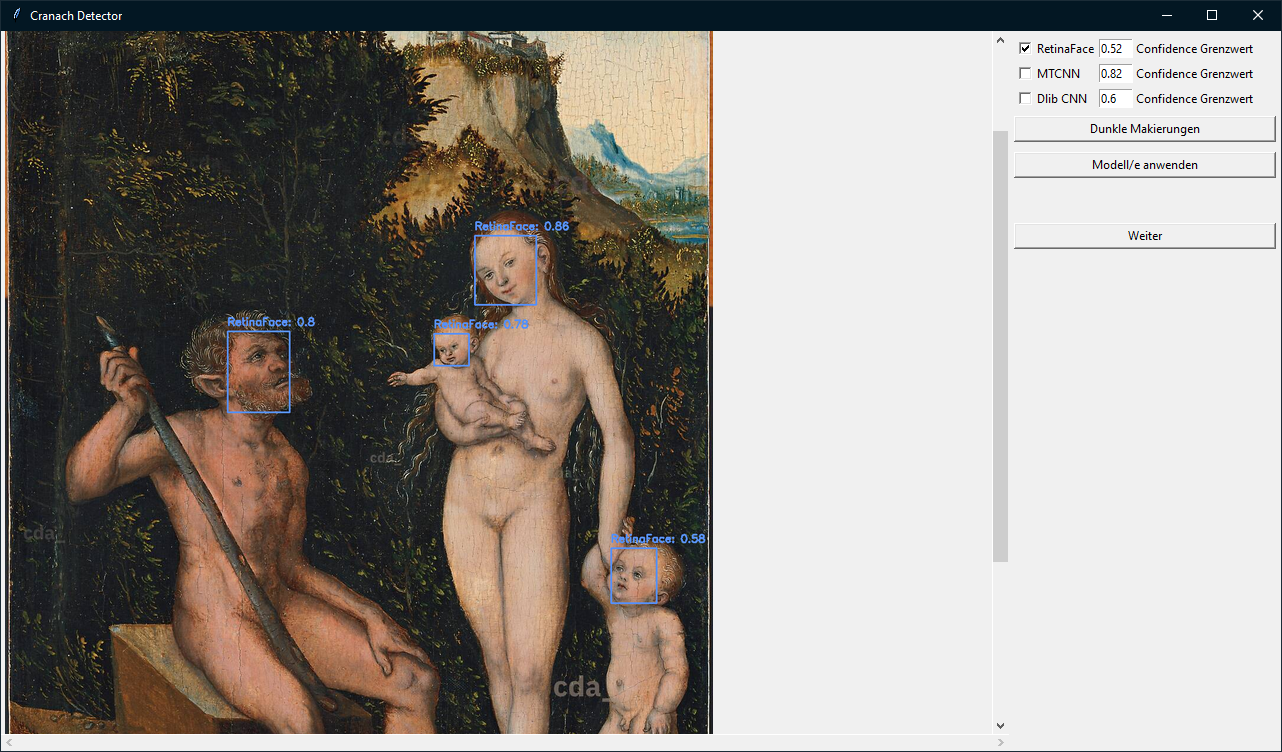
\includegraphics[width=0.9\textwidth]{CranachDetector}
 \caption{GUI von \texttt{cranach\_detector()} (Eigenes Bild)}
 \label{fig:cranachDetector}
\end{figure} 

Auch wenn die \gls{confidence}-Grenzwerte optimiert wurden, kann es dennoch sein, dass bestimmte Bilder andere Werte benötigen. Aus diesem Grund wurde die Möglichkeit hinzugefügt, die \gls{confidence}-Werte während der Laufzeit zu konfigurieren, um für jedes Bild und jedes Modell einzeln Grenzwerte festzulegen, sofern dies erforderlich ist.

Die von den Modellen erkannten Bereiche werden jeweils als Dict in einer Liste gespeichert, mit den Attributen \texttt{x}, \texttt{y}, \texttt{w} (width), \texttt{h} (height), \texttt{model}, \gls{confidence} und \texttt{image\_name}. Diese wird von der Funktion \texttt{cranach\_detector()} nach Durchlaufen aller übergebenen Bilder zurückgegeben. Dabei wird die Liste auch intern in einer Variable gespeichert, um sie mit anderen internen Funktionen wie \texttt{position\_isIntersecting()} und \texttt{area\_isIntersecting()} direkt zu nutzen. Sollte dies nicht ausreichen, kann auf die ausgegebene Liste zurückgegriffen werden. Diese kann dann beispielsweise in eigenen Python-Funktionen weiterverarbeitet werden oder für externe Anwendungen in das JSON-Format überführt werden. Das Format, in dem RetinaFace seine Ergebnisse ausgibt, unterscheidet sich leicht von \gls{mtcnn} und Dlib \gls{cnn}. RetinaFace gibt als Ergebnis die Eckpunkte eines Rechtecks zurück, während die beiden anderen Modelle einen Startpunkt inklusive Breite und Höhe angeben. Um die Arbeit mit den gemeinsamen Ergebnissen der Modelle zu erleichtern, werden die Ergebnisse von RetinaFace in das Format von \gls{mtcnn} und Dlib \gls{cnn} überführt, auch wenn das Format von RetinaFace leichter weiterzuverarbeiten ist. Der Grund, warum Funktionen in diesem Modul dennoch Eingaben im Format \texttt{x}, \texttt{y}, Breite und Höhe erwarten, liegt darin, dass im Frontend eher mit Werten in diesem Format gearbeitet wird.

Die Farben der markierten Gesichter wurden für das Package angepasst, um auch für Menschen mit Farbsehschwäche unterscheidbar zu bleiben. Als Basis für die Auswahl der Farben diente das Paper von \cite{abs-2107-02270}. Gewählt wurden \texttt{(87, 144, 252)} \textcolor{PetroffBlue}{\rule{1em}{1em}} Blau für RetinaFace, \texttt{(248, 156, 32)} \textcolor{PetroffOrange}{\rule{1em}{1em}} Orange für \gls{mtcnn} und \texttt{(228, 37, 54)} \textcolor{PetroffRed}{\rule{1em}{1em}} Rot für Dlib \gls{cnn}. Blau ist die Farbe, die sich am besten eignet, um von anderen unterschieden werden zu können. Sie wurde bewusst für RetinaFace gewählt, da das Modell als Basis dient und so am häufigsten mit den anderen Farben in Kontakt kommt. Allerdings können die gewählten Farben auf bestimmten Bildtypen eine reduzierte Erkennbarkeit aufweisen. Aus diesem Grund wurde die Option hinzugefügt, Markierungen in dunkleren Farben anzeigen zu lassen.

Sollten mehrere Modelle dasselbe Gesicht markieren, wird nur der Bereich mit der geringsten Fläche als gültige Gesichtserkennung beibehalten. Dafür wird überprüft, ob sich zwei markierte Bereiche überschneiden, und die Flächen miteinander verglichen. Wenn der überschneidende Bereich 75\% oder mehr der Fläche des kleineren Bereichs ausmacht, wird der größere Bereich verworfen. So werden möglichst genaue Ergebnisse behalten und vermieden, dass Markierungen von Gesichtern, die nah beieinander liegen, verworfen werden.

Um zu überprüfen, ob eine Position oder ein Bereich auf einem Gesicht liegt, wurden die Funktionen \texttt{position\_isIntersecting()} und \texttt{area\_isIntersecting()} implementiert. Als Argumente erwarten beide Funktionen ein Tupel: (x, y) im Fall von \texttt{position\_isIntersecting()} und (x, y, width, height) bei \texttt{area\_isIntersecting()}, zusammen mit dem Dateinamen eines Bildes, welches zuvor schon einmal von \texttt{cranach\_detector()} bearbeitet wurde, damit intern die markierten Bereiche zur Verfügung stehen. Die Funktionen geben \texttt{True} zurück, sollte sich die Position oder der Bereich auf einem Gesicht befinden.  
Optional kann auch ein Margin angegeben werden, falls ein gewisser Abstand zu Gesichtern eingehalten werden soll. Befindet sich ein Gesicht innerhalb des Margin um den Bereich oder Punkt, gibt die Funktion \texttt{True} zurück.